\section{Segment trees}
\label{sec:segmenet-trees}

Segments tree is another data structure that can be used to answer stabbing queries.
%
It is more general than interval trees as it can process any type of non-intersecting non-vertical line segments, but at the price of increased storage $O(n \log n)$.
%
As we did with interval trees we first shows how segment trees answer stabbing queries and then highlight how to answer window queries.
%

Consider the set of line segments $L = \{ \ell_1, \ell_2, \ell_3, \ell_4, \ell_5\}$ in the following diagram: 

\begin{figure}[h!]
\centering
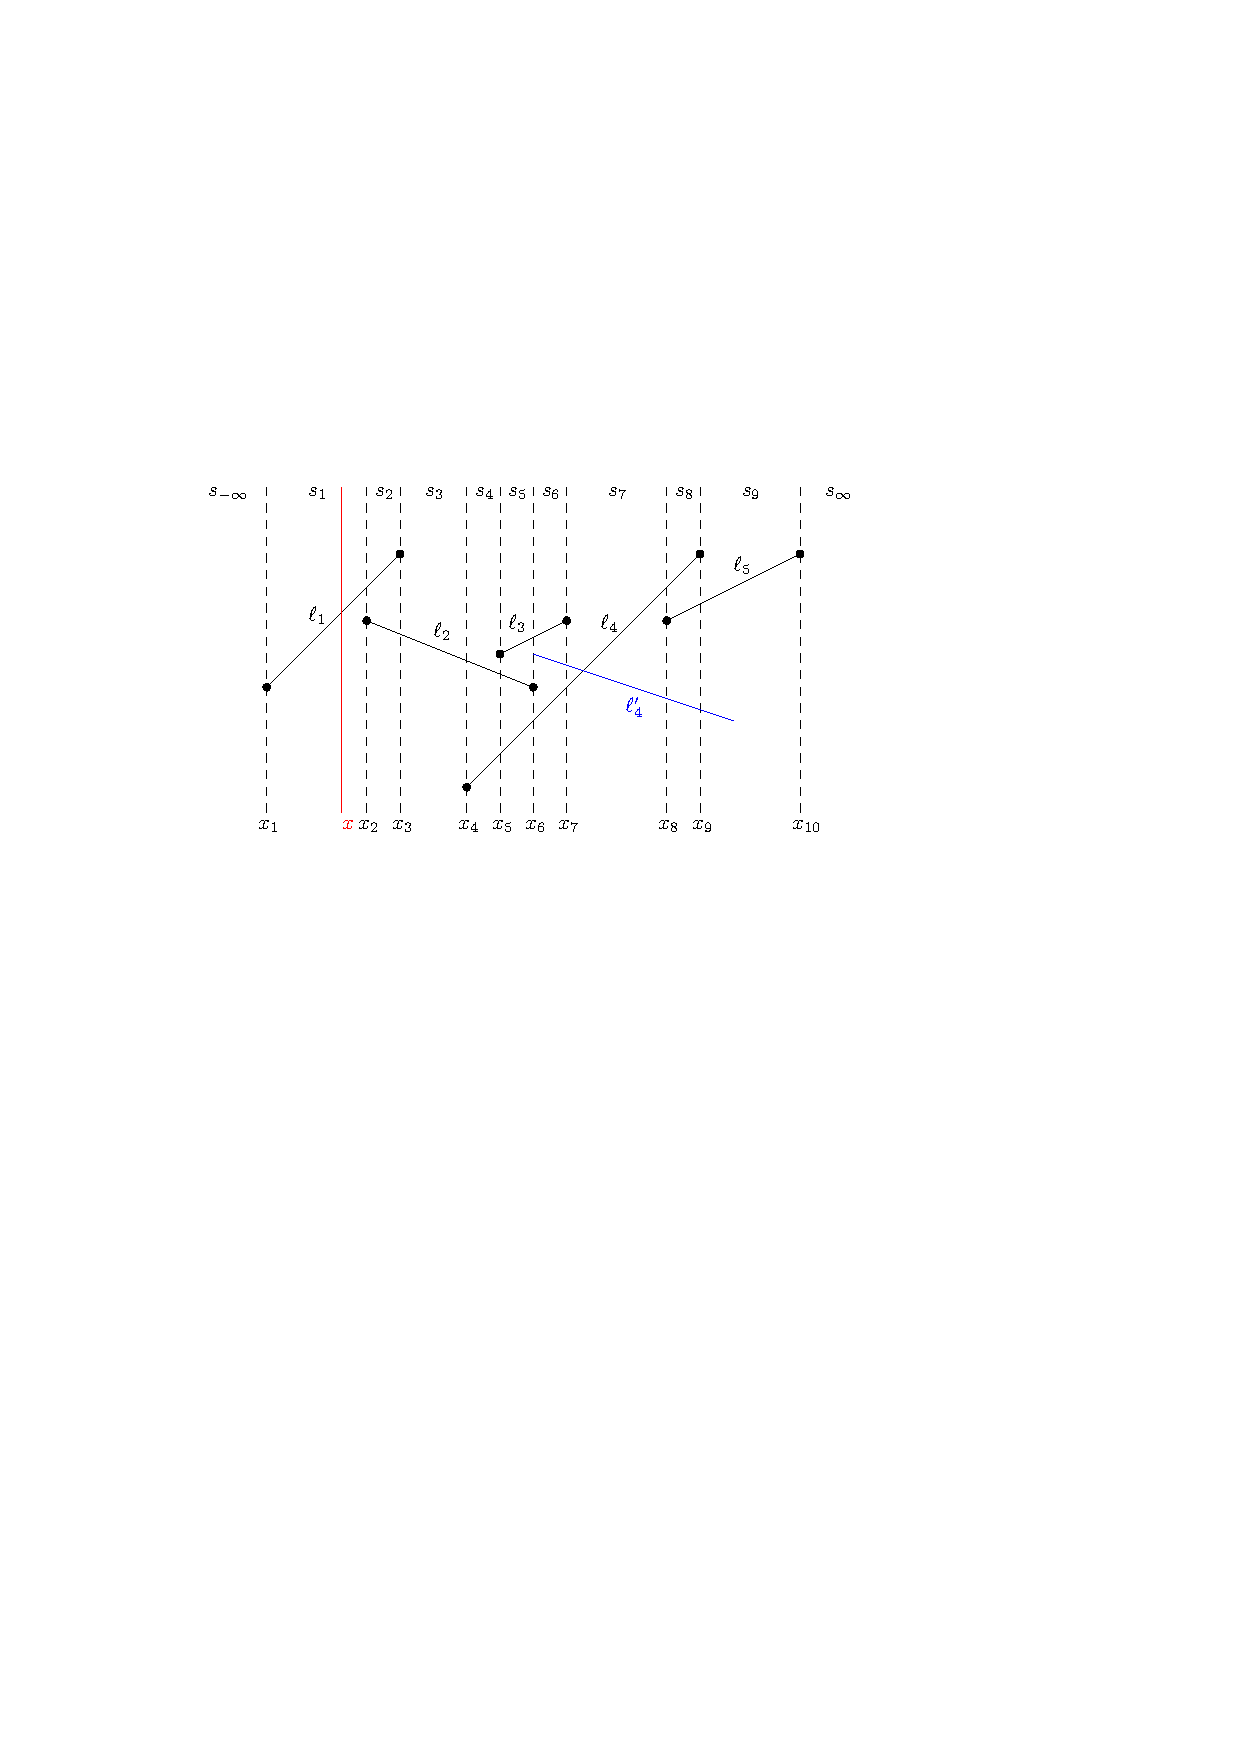
\includegraphics[scale = .8]{ipe/slanted-lines.pdf}
\caption{Set of line segments $L = \{ \ell_1, \ell_2, \ell_3, \ell_4, \ell_5\}$ with slabs $S = \{s_{-\infty},s_1, \dots, s_9, s_{\infty} \}$.}
\label{fig:slanted-lines}
\end{figure}
Observe that we cannot always define a total ordering over slanted line segments that preserves the transitivity property. 
%
For example, if we consider $\ell_5 \leq \ell_4 \leq \ell_2$ then by transitivity we would have $\ell_5 \leq \ell_2$. 
%
On the other hand, if we consider $\ell_2 \leq \textcolor{blue}{\ell'_4} \leq \ell_5$ then we would have $\ell _2 \leq \ell_5$. 
%
However, if we divide the plane into slabs shown by the dashed lines, we can define a total ordering within each slab that is transitive. 

We can build a balanced BST for slabs based on $x$-values of end points with leaves 
\[
S = \{s_{-\infty},s_1, \dots, s_9, s_{\infty} \} ,
\] and internal node $v$ being the union of all slabs within the subtree rooted at $v$. 
%
The root is then all $x$-axis given by the only slab $[-\infty, \infty]$.
%
Next we augment the BST node $v$ with list of line segments $\ell$ that crosses any slab with its subtree but do not cross the parent slab. 

\begin{figure}[h!]
	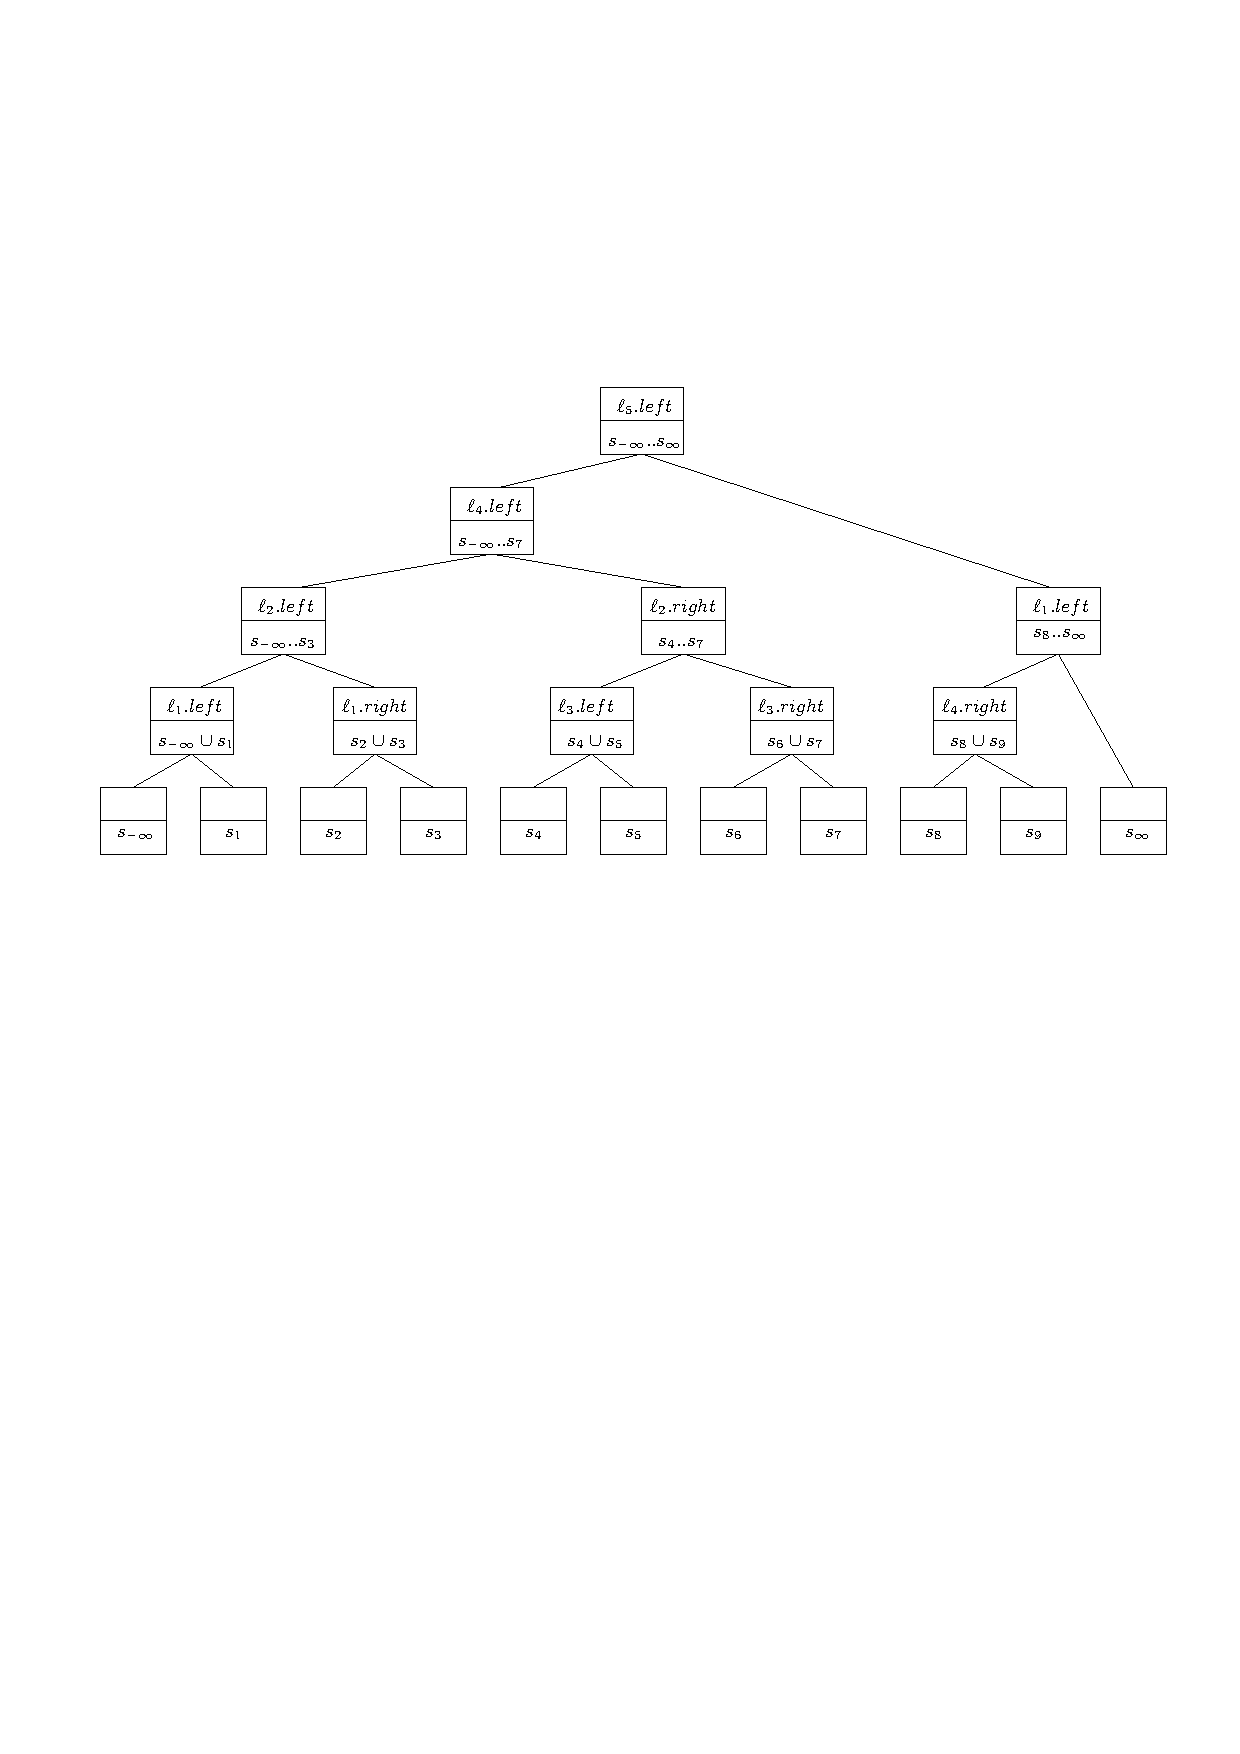
\includegraphics[scale = .8]{ipe/seg-tree-example.pdf}
	\caption{A segment tree for Figure \ref{fig:slanted-lines} with slabs as leaves,  and union of slabs as internal nodes.}
	\label{fig:seg-tree-example}
\end{figure}
%
\paragraph{Invariant} Each line segment $\ell$ is stored in a node of $v$ such that 
\[ [v.x_{left}, v.x_{right}] \subseteq [ \ell.x_{left}, \ell.x_{right}]   \; \wedge \; [parent(v).x_{left}, parent(v).x_{right}] \not \subseteq [\ell.x_{left}, \ell.x_{right}].   \]

\begin{claim}
Each segment will be stored in at most 2 nodes at each level of segment tree.
\end{claim} 

The proof of the claim above can be found in chapter 10 in \cite{Berg:2008}. Based on the result above, the segment tree would take $O(n \log n)$ space because we store at most $2n$ nodes at each level of the BST, and because the tree is balanced. 
%
In order to answer stabbing queries, we locate the slabs that contains the query $\textcolor{red}{q = x}$ from root till leaves level (a single branch) and report all line segments containing $q$.
%
This takes $O(\log n)  $ to locate the leaf node, and $k$ to report the output. Hence, it takes $O(\log n + k)$ to answer stabbing query.

\subsection*{Answering the window query $w = [x_0, \times x_1] \times [y_0 \times y_1 ]$}
In order to answer our original window query $w$, we use 1D range tree to store line segments sorted by $y$-axis. 
%
Note that within each slab in segment tree, we have total ordering of line segments and therefore we can build up a BST without affecting the result.
%
The same analysis for interval trees applies here and we would  have $O(\log n^2 + k)$ query time for segment trees.
